\documentclass[tikz,border=4pt]{standalone}
\usepackage{amsmath}
\usetikzlibrary{calc}
\begin{document}
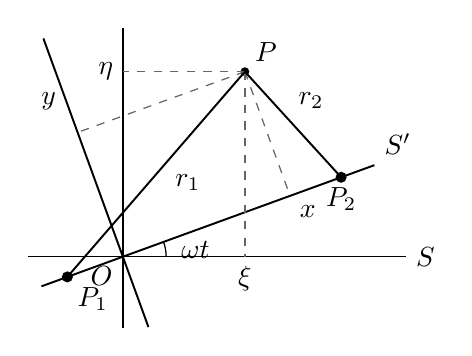
\begin{tikzpicture}[>=stealth, thick, scale=1.0]
  % Inertial frame S (xi, eta)
  \draw[line width=0.5pt] (-1.2, 0) -- (3.6, 0) node[right] {$S$};
  \draw[line width=0.5pt] (0, -0.9) -- (0, 2.9);
  \node[below left] at (0, 0) {$O$};

  % Rotating frame S' (x, y) rotated by angle 20 deg
  \def\ang{20}
  \draw[line width=0.7pt] (\ang:-1.1) -- (\ang:3.4) node[above right] {$S'$};
  \draw[line width=0.7pt] ({\ang+90}:-0.95) -- ({\ang+90}:2.95);
  \node[left] at ({\ang+90}:2.1) {$y$};

  % Points P1 (-mu2 a, 0) and P2 (mu1 a, 0) on x-axis
  \coordinate (P1) at (\ang:-0.75);
  \coordinate (P2) at (\ang:2.95);
  \fill (P1) circle (2.0pt) node[below right] {$P_1$};
  \fill (P2) circle (2.0pt) node[below] {$P_2$};

  % Point P in S-frame: (1.55, 2.35)
  \coordinate (P) at (1.55, 2.35);
  \fill (P) circle (1.6pt) node[above right] {$P$};

  % Projections onto S axes (xi, eta)
  \draw[dashed, line width=0.45pt, black!60] (P) -- (1.55, 0) node[below, black] {$\xi$};
  \draw[dashed, line width=0.45pt, black!60] (P) -- (0, 2.35) node[left, black] {$\eta$};

  % Projections onto S' axes (x, y)
  % x-coord along angle 20: 1.55*cos(20) + 2.35*sin(20) = 1.4565 + 0.8037 = 2.260
  % y-coord along angle 110: -1.55*sin(20) + 2.35*cos(20) = -0.5301 + 2.2083 = 1.678
  \coordinate (Px) at (\ang:2.26);
  \coordinate (Py) at ({\ang+90}:1.68);
  \draw[dashed, line width=0.45pt, black!60] (P) -- (Px) node[below right, black] {$x$};
  \draw[dashed, line width=0.45pt, black!60] (P) -- (Py);

  % Segments r1 = P1--P and r2 = P2--P
  \draw[line width=0.7pt] (P1) -- (P);
  \node[below right] at ($(P1)!0.55!(P)$) {$r_1$};
  \draw[line width=0.7pt] (P2) -- (P);
  \node[above right] at ($(P2)!0.55!(P)$) {$r_2$};

  % Angle omega t
  \draw[line width=0.45pt] (0.55, 0) arc (0:\ang:0.55);
  \node[right] at (8.5:0.62) {$\omega t$};
\end{tikzpicture}
\end{document}
